\documentclass[Rapport/Rapport_main.tex]{subfiles}
\begin{document}
\section{RPi}
I dette segment af rapporten vil de væsentligste dele af RPiApp blive forklaret. Applikationen kan opdeles i tre dele: Et system til håndtering af trådsikret kommunikation og ressourcer, en Web applikation og en grafisk brugeroverflade. 
\subsection{RPiApp - GameController}
I dette afsnit fokuseres på softwarens 'event driven' arkitektur, trådkommunikation og logiske operationer - systemet består af flere klasser men benævnes som GameController systemet. De vigtigste klasser: GameController, Playerside, BallDispenser, I2C og UserInfo. En uddybende beskrivelse af klasserne kan findes i afsnittet "XX"
\subsubsection{Softwaredesign}
\textbf{Event Driven Arkitektur:} \\
Beer Pong er et eventbaseret spil. Det omhandler masser af asynkrone handlinger; når der rammes ned i en kop, fjernelse af kop, indsættelse af mønt mm. Det er således utrolig vigtig, at vores system kan opfange alle disse asynkrone events. Selvom alle handlingerne fra brugeren er asynkrone, ønsker vi stadigt at interagere med handlingerne sekventielt. Dette er en vigtig faktor, da hvis en bruger laver to eventhandlinger inden for en kort tidsramme, skal vi sikre at systemet når at reagere på begge handlinger. En af måderne for at opnå dette er reaktiv programmering: Vi ønsker at opdatere vores system med det samme brugeren interagere med det. \\
Dette problem løses ved event driven arkitektur: Et system som reagerer ud fra signaler og tilstande fra aktører/delsystemer. Det er essentielt at de asynkrone signaler afvikles sekventiel og i et trådsikkert system. Her anvendes klassen MsgQueue, som er baseret på Producer / Consumer idiomet. 
\begin{figure}[H]
    \centering
    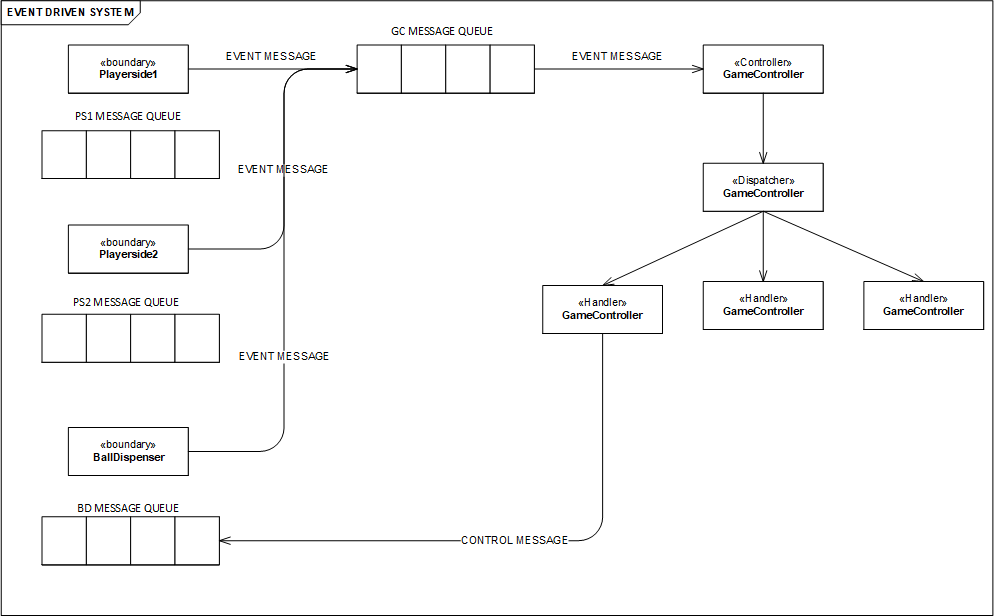
\includegraphics[width=1\textwidth]{Softwaredesign/RPiApp/graphic_RPi/EDS.png}
    \caption{Skitse af event driven system og MsgQueue system. Hvert boundary klasse har en MsgQueue instans, som er en 'consumer'. De andre klasser, som har tilgang til MsgQueue instansen, kan sende beskeder ved at allokerer besked. Beskeden består af et id og en instans nedarvet fra klassen 'Message'. Som det kan ses på skitsen, er der ingen klasser som har direkte 'kontakt' med hinanden, alt kommunikation sker gennem MsgQueues}
   \label{fig:Sketch_Event}
\end{figure}
MsgQueue-systemet indfører også et trådsikret system, da alt data sendt gennem systemet er indkapslet af mutex'er. Desuden allokeres og deallokeres nedarvede beskeder af base klassen Message dynamisk - denne form for hukommelsesadministration sikre at ressourcerne bliver frigivet korrekt og der ikke opstår 'resource leaks'. For en mere detaljeret beskrivelse af event driven arkitektur, håndtering af resourser og MsgQueue-systemet henvises til Softwaredesign dokumentet, afsnit "Design af RPiApp - USER SPACE"\footnote{MANGER REF}.\\\\
\textbf{GameController - Controller:}\\
Softwaredesignet for GameController, Playerside, BallDispenser, I2C og UserInfo er dokumenteret i afsnit X i bilaget "Softwaredesign". \\
Controller klassen, GameController, beskrivet kort i Rapporten, da den er essentiel for hele systemet. \\
RPiApp er omfangsrigt program og mange asynkrone handlinger og signaler skal behandles. GameController klassen er samlingspunktet for hele applikationen og indeholde alle de logiske operationer. Den bruger boundary klasserne til at dirigere PSoC-enhederne og GUI.
\begin{figure}[H]
    \centering
    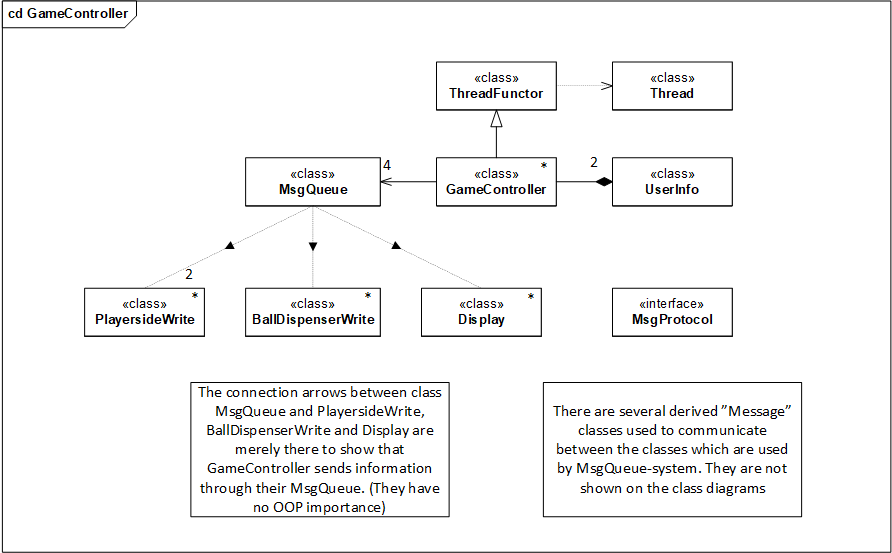
\includegraphics[width=1\textwidth]{Rapport/RPi/graphics/GameController.png}
    \caption{Klasse diagram for GameController. GameController anvender MsgQueue associationerne til at kommunikere med boundary klasserne. Boundary klasserne videreføre alle kommandoer udsendt fra GameController videre til delsystemerne som Playerside enhederne, BallDispenser enheden og GUI.}
   \label{fig:cd_GameController}
\end{figure}

\subsubsection{Implementering}
Softwareapplikation RPiApp er generelt udviklet objektorienteret i sproget C++17. Sproget bruges da det kan kompileres og afvikles på den valgte computerenhed, Rasberry Pi W Zero. C++ bruges til at udvikle det event driven arkitektur og det trådsikret system, men der bruges også elementer af C11 til at få adgang til filoperationer i Kernal Space.

RPiApp's kildekode kan findes i bilaget "XXX"

\subsubsection{Modultest}
Til test af GameController systemet blev white-box testing benyttet. Her blev de interne strukture testes, primært MsgQueue trådkommunikationen. Trådkommunikationen blev testet ved at sende dynamisk allokeret beskeder mellem klasserne, som indeholdt en MsgQueue (Producer / Consumer problemet). \\
Black-box testning blev også brugt til at teste grænsefladerne for de øvrige del-systemer: Playerside-enhederne og BallDispenser-enheden. Grænsefladen til begge enheder består af i2c kommunikation. Da det ikke er muligt at få adgang til Kernal Space operationer fra User Space, blev filoperationerne blot testet. \\\\
Begge tests er nærmere beskrevet i afsnittet "XX" i bilag "Modeltest"
%%Mangler at lave black-box testing i modultest dokumentet


\subsection{RPiApp - WebPage}
Dette afsnit omhandler boundary-klassen WebPage. I Beer Pong bordets RPi Zero W er der installeret en Apache web server, som er en populær webserver applikation, der gør det muligt at hoste hjemmesider.\textcolor{orange}{ref} Systemet giver brugerne mulighed for at tilgå hjemmesiden via smartphone, eller et andet mobilt device og indtaste holdnavne, brugernavne og holdfarve. WebPage er i denne forbindelse anvendt som en samlet betegnelse for alt, hvad der har med hjemmesiden at gøre. I virkeligheden består den af en klientside og serverside, som kommunikerer internt gennem et WebSocket API. 

\subsubsection{Softwaredesign}
Klassediagram med beskrivelse

\\\\\textbf{Websocket}
\\Web kommunikation forløber typisk ved, at der etableres et forhold mellem client og server, som er baseret på anmodninger og svar. Client kan eksempelvis være en web browser og server en applikation, som hoster en hjemmeside. En ofte anvendt protokol til denne form for kommunikation er HTTP.\textcolor{orange}{ref} HTTP er en request-response protokol, og kommunikationen er som regel initieret af client. Client sender en HTTP request eller besked til serveren, og server svarer igen med et HTTP response, som både kan indeholde status information, eller andet indhold, der er anmodet om.\textcolor{orange}{ref} \\Ved at opdatere HTTP forbindelsen til en WebSocket kan der etableres en vedvarende forbindelse mellem client og server. Dermed kan der sendes beskeder frem og tilbage over en enkelt TCP port, uden at client først skal sende en forespørgsel. Kommunikationen kan betegnes som full-duplex og graden af overhead er sænket.\textcolor{orange}{ref} Der oprettes et egentligt WebSocket objekt, og der er fire events associeret med dette, som beskrives nærmere i afsnit \textcolor{orange}{ref} i bilag "Dokumentation". 

\\\\\textbf{Client}
\\Client beskriver hjemmesidens interface. Det er her defineret, hvordan hjemmesiden skal præsentere sig i web browseren og WebSocket API beskrevet i forrige afsnit er implementeret. Under initieringen oprettes WebSocket objektet og de event handlers, som er en del af API er ligeledes beskrevevet her. Når data skal sendes mellem client og server skal det ske i tekstformat. Der er derfor designet en løsning, hvor spillerne har mulighed for at indtaste holdnavne og brugernavne samt vælge holdfarver på track bars for henholdsvis hold 1 og hold 2. Når der trykkes på en 'Start' knap på hjemmesiden genereres et event, som medfører, at alle brugerinputs konkateneres til én tekststreng og sendes til serveren.

\\\\\textbf{Server}
\\Serversiden har til opgave at modtage og behandle førnævnte data fra client og er implementeret som en C++-klasse. Den lytter aktivt på den relevante port, og når tekststrengen modtages bliver denne indlæst i en buffer og separaret på passende vis. Informationerne opbevares i en STL container og anvendes til at sætte members på to objekter af UserInfo klassen, team1\_ og team2\_. Disse objekter skal sendes til GameController klassen, og hertil anvendes det tidligere beskrevne event drevne system med Messages og MsgQueues. WebPage har derfor kendskab til GameControllers MsgQueue, men det omvendte gør sig ikke gældende. Hvis GameController først sendte en request besked for herefter at modtage objekterne i en responsebesked fra server kunne der hurtigt opstå komplikationer. Der blev forudset problemer med race conditions og problematisk adfærd. Kommunikationen mellem server og GameController er derfor bevidst gjort envejs så dette undgås, og dermed sikres det også, at GameController altid arbejder på de nyeste brugerinputs.

\subsubsection{Implementering}
Webserver hostes som bekendt af en RPi Zero W. Den er derfor implementeret som en C++-klasse i sproget C++17. Hjemmesidens interface beskrevet i afsnittet client er implementeret med det såkaldte 'markup language' HTML5 i kombination med Cascading Style Sheets (CSS). Script-sproget Javascript anvendes til at implementere hjemmesidens dynamiske elementer samt WebSocket API. For flere informationer vedrørende implementeringen henvises til kildekoden i bilag \textcolor{orange}{ref}.

\subsubsection{Modultest}
Se bilag.

\subsection{I2C\_interruptDriver}
\subfile{Rapport/RPi/I2C_interruptDriver/Design.tex}
\subfile{Rapport/RPi/I2C_interruptDriver/Implementering.tex}
\subfile{Rapport/RPi/I2C_interruptDriver/Modultest.tex}

\subsection{RPiApp - GUI}
\subfile{Rapport/GUI/GUI_software_rapport.tex}
\subsubsection{Softwaredesign}
\subsubsection{Implementering}
\subsubsection{Modultest}


\end{document}